\documentclass[../main.tex]{subfiles}

\begin{document}

\section{Introductie en overzicht}%
\label{sec:introductie_en_overzicht}

Er worden min of meer 2 handboeken gevolgd "Modern Particle Physics, Thomson, Cambridge" en "Introduction to Elementary Particle Physics,  Bettini, Cambridge, 2008". De boeken zijn veel gestructureerd dan de cursus. De cursus volgt meer de chaotische structuur van de geschiedenis van de experimenten. Hierdoor krijg je ook meer inzicht hoe de experimenten verlopen en dat het niet altijd even logisch hoort te zijn. Op dit ogenblik weten we nog zeker niet alles en zien nog niet altijd de logica. Bij experimenten wordt er altijd in het duister getast. De bedoeling van deze master cursus is deels om de mensen in de war te brengen en kritisch na te denken.\\
De cursus bestaat uit 12 hoofdstukken waarbij je het meest uitkijkt naar het laatste hoofdstuk. Deze bespreekt de fysica die we nog niet kennen, met andere woorden niet het Standaard Model.

\subsection{High energy physics}%
\label{sub:high_energy_physics}
Hier wordt er gekeken naar de fundamentele constituenten van de materie en naar de interactie tussen hen. Met andere woorden kijken we naar materie deeltjes en naar krachten.

\begin{table}[h]
    \centering
    \caption{Fundamentele materie}
    \label{tab:fund_mat}
    \begin{tabular}{cc|c|ccc}
        \multicolumn{1}{c}{\multirow{2}{*}{Leptons}} & $\nu_e$ & $\nu_\mu$ & $\nu_\tau$ & $q=0$ & neutrinos \\
        \multicolumn{1}{c}{}                         & $e^-$ & $\mu^-$ & $\tau^-$ & $q=-1$ & charged leptons \\ \hline
        \multirow{2}{*}{quarks}                      & $u$ & $c$ & $t$ & $q=+2/3$ & up-type \\
                                                     & $d$ & $s$ & $b$ & $q=-1/3$ & down-type
    \end{tabular}
\end{table}

Dat er zowel 6 leptons als quarks zijn is waarschijnlijk geen toeval maar in principe hoeft dit niet. Er zijn bijna geen relaties tussen leptonen en quarks op dit moment. Enkel via de Coulomb kracht zullen deze met elkaar interageren. De leptonen en quarks worden opgedeeld in 3 generaties met als enig verschil tussen de generatie de massa. Waarbij het zwaarder deeltje zal kunnen vervallen naar het lichtere deeltje met zelfde kwantum getallen. Al deze deeltjes vermeld in tabel \ref{tab:fund_mat} zijn elementaire deeltjes met spin 1/2 en zijn dus fermionen. Met als gevolg dat deze de Dirac vergelijking volgen en we ze kunnen zien als punt deeltjes.\\
Leptonen kunnen vrij zijn. In tegenstelling zijn quarks nooit vrij. Deze binden tot composiet deeltjes (hadrons):

\begin{itemize}
    \item baryons: $\left|B\right>=\left|q_1q_2q_3\right>$
    \item anti-baryons: $\left|\overline B\right>=\left|\overline q_1\overline q_2\overline q_3\right>$
    \item mesons: $\left|M\right>=\left|q_1q_2\right>$
    \item anti-mesons: $\left|\overline M\right>=\left|\overline q_1\overline q_2\right>$
\end{itemize}

De reden voor deze "confinement" is dat alle deeltjes wit moeten zijn. Het bewijs hiervoor is nog niet volledig uitgewerkt. Dit is een probleem van quantum chromo dynamics (=QCD). De laatste jaren zijn er ook penta- ($\left|P_c^+\right>=\left|uudc\overline c\right>$) en tetraquarks ($\left|Z\right>=\left|c\overline c d\overline u\right>$) gevonden.

\subsection{Discovering the electron}%
\label{sub:discovering_the_electron}

In 1897 heeft J.J. Thomson het electron voor het eerste keer ontdekt met volgende eigenschappen:
\begin{itemize}
    \item $q_e = -1.602\cdot 10^{-19}$C
    \item $m_e = 0.9\cdot 10^{-31}$kg
    \item $s = \frac{1}{2}\hbar = 0.5\cdot 10^{-34}$J.s
\end{itemize}

\begin{figure}[h]
    \centering
    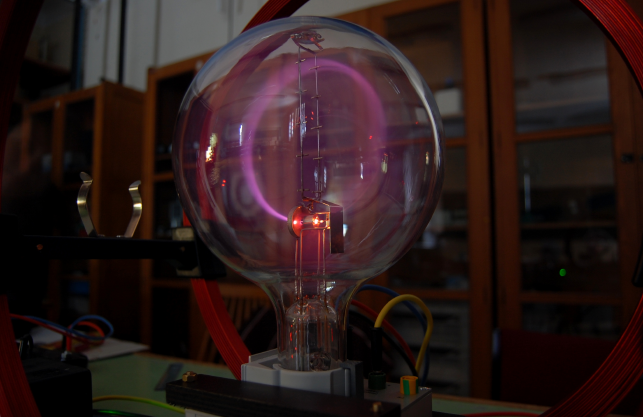
\includegraphics[width=0.8\linewidth]{introduction_and_review/elec_disc.png}
    \caption{The discovery of the electron}%
    \label{fig:elec_disc}
\end{figure}

Voor ons eigen gemak voeren we nieuwe eenheden in:
\begin{itemize}
    \item $Q_e = -1$
    \item $m_e = 0.511$MeV (gebruik $E=mc^2$)
    \item $s=\frac{1}{2}$
\end{itemize}
Hierbij wordt gebruik gemaakt van de natuurlijke eenheden $\hbar = c = 1$. Hierbij zeggen we dat $[T]=s$ en definiëren we de lengte zodat $c=1$ en de massa zodat $\hbar = 1$. Zo krijgen we de volgende relaties:
\begin{equation}
    \begin{aligned}
        \label{eq:nat_units}
        [L]&=[T]\\
        [M]=[E]&=[P]=[L^{-1}
    \end{aligned}
\end{equation}
De gevolgen hiervan zijn dat:
\begin{equation}
    \begin{aligned}
        \label{eq:nat_units_gevolgen}
        1 \text{MeV} &= 1.52 \cdot 10^{21} s^{-1}\\
        1 \text{MeV}^{-1} &= 197\text{fm}\\
        1 \text{ps}^{-1} &= 0.65 \text{meV}\\
        1 \text{m} &= 5.07\cdot 10^6 \text{eV}^-1
    \end{aligned}
\end{equation}
De enige die je hiervan onthoudt is de 2de. Deze komt uit $\hbar c = 197$MeV.fm. Voor de relativistische kinematica krijgen we:
\begin{equation}
    \begin{aligned}
        \label{eq:rel_kin}
        \beta = v\\
        E^2 = m^2 + |\vec{p}|^2
    \end{aligned}
\end{equation}

\subsection{Interacties}%
\label{sub:interacties}

Er zijn op dit moment 5 krachten: elektrisch, magnetisch, zwak, sterk en gravitationeel. We zouden dit graag reduceren tot 1 fundamentele kracht in de "Theory of Everything" maar dit is nog niet gelukt. De koppelingsconstantes van deze krachten kan je vinden in tabel \ref{tab:coupling_constants}.
\begin{table}[h]
    \centering
    \caption{Koppelingsconstantes}
    \label{tab:coupling_constants}
    \begin{tabular}{cccc}
                & rel. strength & works on              & exch. part. \\
        \hline
        strong  & 1             & quarks                & gluons \\
        EM      & $10^{-2}$     & q + charged leptons   & photon \\
        weak    & $10^{-7}$     & q + l + $\nu$         & $W^+,W^-,Z^0$
    \end{tabular}
\end{table}

\subsection{Deeltjes experimenten}%
\label{sub:deeltjes_experimenten}

Deze cursus zal vooral uitweiden over experimenten om grotere beelden te maken van de theorie. Wat staat er in de experimentele grafieken?\\
Het is belangrijk een hoge resolutie nodig om de kleine deeltjes te zien. Het is nodig om hoge center of mass energieën te hebben om nieuwe zware deeltjes te ontdekken.
\begin{equation}
    \begin{aligned}
        \label{eq:E_cm}
        E_{cm} = \sqrt{s}
    \end{aligned}
\end{equation}
In een collider met vaste targets is $s=E_{beam}$ voor colliding beams is $s=E_{beam}^2$.

\subsection{Mandelstam-variables}%
\label{sub:mandelstam_variables}

\begin{equation}
    \begin{aligned}
        \label{eq:mandelstam}
        a+b&\rightarrow c+d\\
        s=(p_a&+p_b)^2\\
        s=(E_a&+E_b)^2-(\vec{p}_a + \vec{p}_b)^2\\
        t=(E_c&-E_a)^2-(\vec{p}_c - \vec{p}_a)^2\\
        u=(E_d&-E_a)^2-(\vec{p}_d - \vec{p}_a)^2\\
    \end{aligned}
\end{equation}
s is een Lorentz invariante grootheid en moet geconserveerd blijven tijdens de collisies. Naast de $s$ variabele bestaan ook $t$ het overgebrachte 4-moment $a-c$ en $u$ van $a-d$.\\
Dit is ooit een examenvraag geweest om te bewijzen dat $s+t+u=m_a^2+m_b^2+m_c^2+m_d^2$.
\begin{equation}
    \begin{aligned}
        \label{eq:stu_bewijs}
        s&=p_a^2+p_b^2+2p_a\cdot p_b\\
        t&=p_a^2+p_c^2-2p_a\cdot p_c\\
        u&=p_a^2+p_d^2-2p_a\cdot p_d\\
         &\downarrow\\
        s+t+u&=p_a^2+p_b^2+2p_a\cdot p_b + p_a^2+p_c^2-2p_a\cdot p_c + p_a^2+p_d^2-2p_a\cdot p_d\\
             &=m_a^2+m_b^2+m_c^2+m_d^2+(2p_1^2+2p_a\cdot p_b-2p_a\cdot p_c-2p_a\cdot p_d)\\
             &\downarrow \text{vergelijking (\ref{eq:stu_help}) en behoud van momentum}\\
             &=m_a^2+m_b^2+m_c^2+m_d^2
    \end{aligned}
\end{equation}

\begin{equation}
    \begin{aligned}
        \label{eq:stu_help}
        2p_1^2+2p_a\cdot p_b-2p_a\cdot p_c-2p_a\cdot p_d = 2p_1\cdot (p_1 + p_2 - p_3 -p_4) = 0
    \end{aligned}
\end{equation}
Hierbij kunnen we deze vergelijking gelijk stellen aan $0$ omdat $p_1 + p_2 - p_3 -p_4 = 0$.\\
Deze variabelen zijn makkelijk om de s, t en u kanalen in deze botsingen te beschrijven.

\begin{figure}[h]
    \centering
    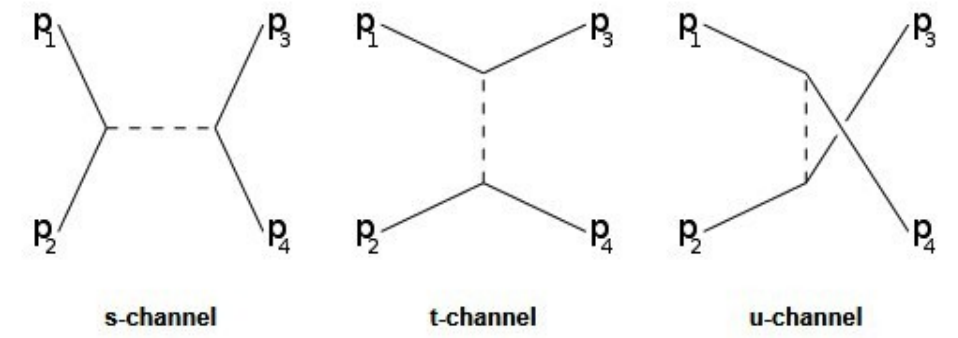
\includegraphics[width=0.8\linewidth]{introduction_and_review/kanalen.png}
    \caption{Mogelijke kanalen tijdens botsingen}%
    \label{fig:kanalen}
\end{figure}

Kijken we naar de werkzame doorsnedes van deze kanalen zien we:
\begin{equation}
    \begin{aligned}
        \label{eq:kanalen_doorsnede}
        \sigma&\sim\frac{1}{E^2}\\
        \text{s kanaal: }&\sim\frac{1}{s}\\
        \text{t kanaal: }&\sim\frac{1}{t}\\
        \text{u kanaal: }&\sim\frac{1}{u}
    \end{aligned}
\end{equation}
Als voorbeeld $e^+ +e^- \rightarrow e^+ + e^-$:\\
\begin{minipage}[c]{0.5\textwidth}
    \begin{center}
        \feynmandiagram[horizontal=a to b]{
            a -- [boson] b,
            i1 [particle=\(e^-\)] -- [fermion] a,
            a -- [fermion] i2 [particle=\(e^+\)],
            f1 [particle=\(e^+\)] -- [fermion] b,
            b -- [fermion] f2 [particle=\(e^-\)],
        };
    \end{center}
\end{minipage}\noindent
\begin{minipage}[c]{0.5\textwidth}
    \begin{center}
        \feynmandiagram[vertical=a to b]{
            a -- [boson] b,
            i1 [particle=\(e^+\)] -- [fermion] a,
            a -- [fermion] i2 [particle=\(e^+\)],
            f1 [particle=\(e^-\)] -- [fermion] b,
            b -- [fermion] f2 [particle=\(e^-\)],
        };
    \end{center}
\end{minipage}
Het u kanaal is hier niet mogelijk omdat we met verschillende deeltjes werken. Het u kanaal is enkel mogelijk als we met gelijke deeltjes werken. De reden hiervoor is dat de vertex van $e^-$ naar $e^+$ niet bestaat.

\subsection{Acceleratoren}%
\label{sub:acceleratoren}

Er zijn verschillende acceleratoren: 
\begin{itemize}
    \item lepton colliders: $e^+e^-$, wordt gelimiteerd door de synchroton straling
    \item assymetrische colliders: $e^-p$
    \item hadron colliders: $p\overline p$ of $pp$, nadeel dat deze botsingen veel complexer zijn
\end{itemize}

\subsection{Detectoren}%
\label{sub:detectoren}

Deze bestaan uit een uienstructuur.

\begin{figure}[h]
    \centering
    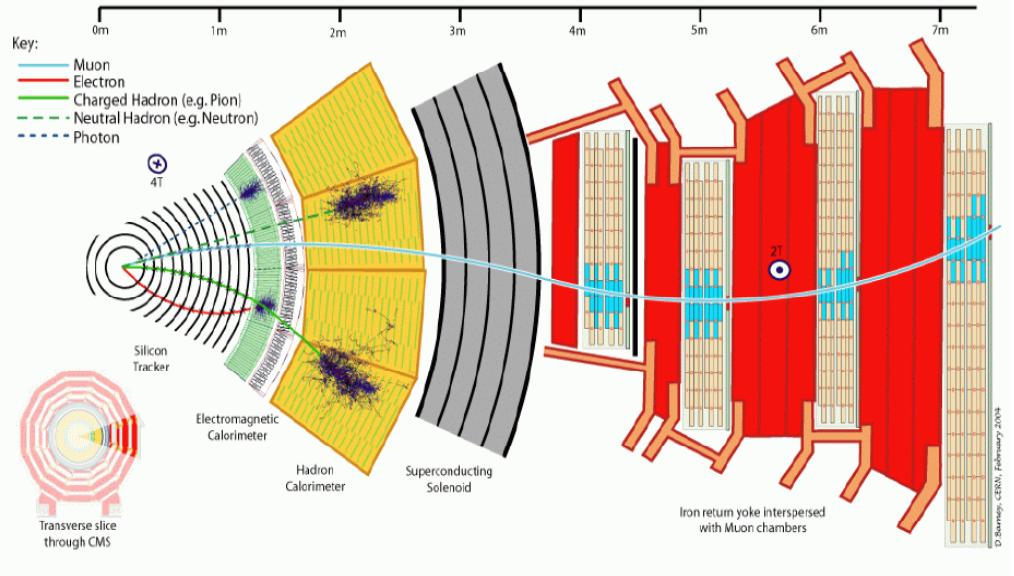
\includegraphics[width=0.8\linewidth]{introduction_and_review/detector.png}
    \caption{Detector}%
    \label{fig:detector}
\end{figure}

De verschillende lagen zijn in volgorde:
\begin{itemize}
    \item centraal, tracker: deeltjes die afbuigen in EM veld
    \item magnetische calorimeter
    \item hadronische calorimeter
    \item magneten
    \item muon detectoren
\end{itemize}

\subsection{Energie verlies}%
\label{sub:energie_verlies}

Een geladen deeltje zal met het bewegen door de detector energie verliezen. De Bethe-Bloch functie beschrijft het gemiddelde energieverlies voor door ionisatie.
\begin{equation}
    \begin{aligned}
        \label{eq:bethe_bloch}
        -\frac{dE}{dx}=K\frac{\rho Z}{A}\frac{z^2}{\beta^2}\left[\ln\left(\frac{2m_ec^2\gamma^2\beta^2}{I}-\beta^2\right)\right]
    \end{aligned}
\end{equation}

\begin{figure}[h]
    \centering
    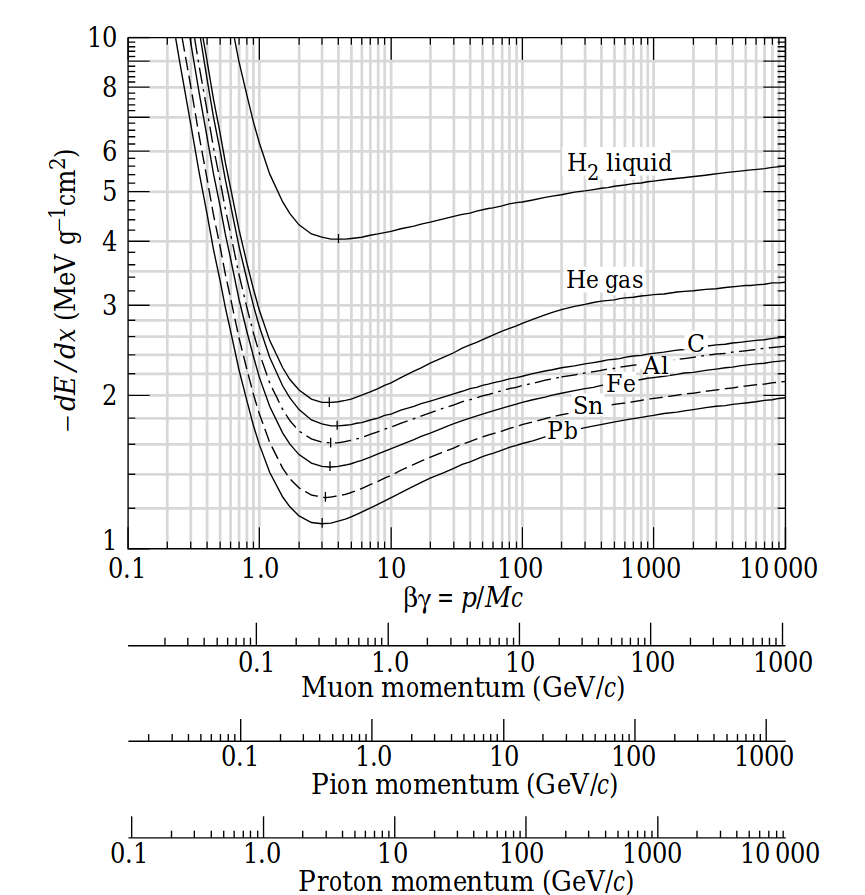
\includegraphics[width=0.8\linewidth]{introduction_and_review/bethe_bloch.png}
    \caption{Bethe bloch functie}%
    \label{fig:bethe_bloch}
\end{figure}
In figuur \ref{fig:bethe_bloch} gegeven in de zone tussen $0.1$ en $10$. Dit is door coulomb interactie met atomen. De $\beta^2$ factor ook wel de relativistische rise is het gevolg van Brehm stralung waarbij deeltje worden afgebogen door het atoom en een hoog energetisch foton uitsturen.\\
De muonen bevinden zich meestal in de zone waar het energieverlies het laagste is en noemen we dan ook minimum ionising particles. Elektronen gaan heel veel fotonen afstralen en verliezen heel veel energie. Hadronen zullen naast het ioniseren ook sterke interacties ondergaan. Hierdoor verliezen we het originele deeltje en worden secondaire hadronen gemaakt.

\subsection{Deeltjes detectoren}%
\label{sub:deeltjes_detectoren}

We gaan de verschillende deeltjes die gecreerd zijn tracken van de geladen deeltjes, zowel de richting als hun momentum. Dit wordt gedaan de hand van ionisatie. We doen ook aan calorimetrie wat een destructieve detectiemethode is. Ten laatste buiten de calorimeters worden de muonen gedetecteerd. De werking voor de verschillende detectoren gaat als volgt:
\begin{itemize}
    \item Tracking detectoren: Een deeltje beweegt door een gebied met gas die de gasatomen ioniseert. In dit gas is een hoogspanningsveld aanwezig zodat de geladen atomen zullen driften richting de anode of kathode en zo een signaal bekomen. Door een nauw grid aan anodes en kathodes aan te leggen kan dit heel nauwkeurig gemeten worden. Dit kan ook met een halfgeleider en krijg je elektron-gat paren in plaats van electron-ion paren.
        \begin{figure}[h]
            \centering
            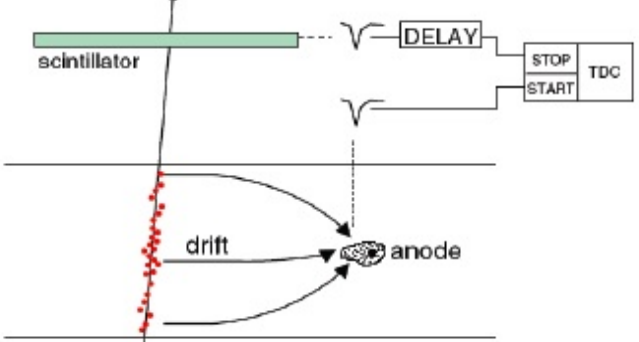
\includegraphics[width=0.8\linewidth]{introduction_and_review/tracking_detector.png}
            \caption{Tracking detector}%
            \label{fig:tracking_detector}
        \end{figure}
    \item Calorimeter detectoren: Dit is meestal een kristal waar de energie van de deeltjes meestal omgezet worden in zichtbaar licht die kan gedetecteerd worden.
\end{itemize}

\subsection{Event reconstructie}%
\label{sub:event_reconstructie}

Als voorbeeld de top pair productie om aan te tonen dat de detectie niet zo makkelijk is als het lijkt.
\begin{equation}
    \begin{aligned}
        \label{eq:top_prod}
        pp \rightarrow &t\overline t X\\
                       &t\rightarrow W^+b\rightarrow \mu^+\nu b\\
                       &\overline t \rightarrow W^-b\overline b \rightarrow q\overline q' \overline b\\
        pp \rightarrow &b\overline bq\overline q' \nu\mu
    \end{aligned}
\end{equation}
De X in deze productie zijn de overige 100 tot 1000den deeltjes die geproduceerd kunnen worden door 1 botsing. Hieruit moeten de correcte deeltjes uit gedetecteerd worden wat natuurlijk niet eenvoudig is. Hierboven hebben we een groot probleem bij het onderzoeken van de top quark dat deze een heel korte levensduur heeft. Uiteindelijk krijgen we hieruit 4 ``jets'' van de quarks, een $\mu$ en een deel missende energie waarnemen. Om de top quarks te reconstrueren gaan we proberen de b-jets proberen taggen. Door het gebruik van een hermetische detector zal het ook mogelijk zijn om de missende energie van de neurtrino's te vinden. Dit kan natuurlijk enkel in de trasversale richting.

\subsection{Cross sectie}%
\label{sub:cross_sectie}

De interactie rate per eenheid van tijd is gegeven door:
\begin{equation}
    \begin{aligned}
        \label{eq:int_rate}
        R_i=\sigma N_t \Phi_b
    \end{aligned}
\end{equation}
met $\sigma$ de cross sectie, $N_t$ het aantal targets in de beam sectie en $\Phi_b$ de beam flux. Kijken we nu bijvoorbeeld naar de protonen die door de detector tracken en kunnen in de elektromagnetische calorimeter botsen met andere deeltjes en verloren gaan. Dit kan gezien worden in de volgende vergelijkingen.
\begin{equation}
    \begin{aligned}
        \label{eq:beam_intensity}
        dI(z) = -dR_i &= -\sigma\Phi_b(z)dN_t\\
                      &= -\sigma\frac{I(z)}{A}n_tAdz\\
        \Rightarrow\frac{dI(z)}{I(z)}&=-\sigma n_tdz\\
        \Rightarrow I(z)&=I_0e^{-n_t\sigma z}
    \end{aligned}
\end{equation}
Uit de exponent die we juist hebben berekend kunnen we de absorptie lengte bepalen: $L_{abs}=1/(n_t\sigma)$. Voor protonen met energieën van een aantal TeV zullen een $L_{abs}$ van ongeveer $10$cm hebben in detectoren. De luminositeit $\mathcal{L}$ is gegeven door:
\begin{equation}
    \begin{aligned}
        \label{eq:luminositeit}
        \mathcal{L} &= \frac{R_i}{\sigma} = \Phi_b N_t = \frac{N_bN_t}{A}\\
        [\mathcal{L}] &= [L^{-2}T^{-1}]
    \end{aligned}
\end{equation}
Het handige aan $\mathcal{L}$ is dat deze grootheid gekend is omdat we het aantal target deeltjes in de bundel en de flux van de bundelonder controle hebben. Dit samen met het aantal uitgaande deeltjes kunnen we zien wat de werkzame doorsnede is. De geintegreerde luminositeit wordt ook veel gebruikt: $\int \mathcal{L}dt$.

\subsection{Differentiële cross sectie}%
\label{sub:differentiele_cross_sectie}

\begin{figure}[h]
    \centering
    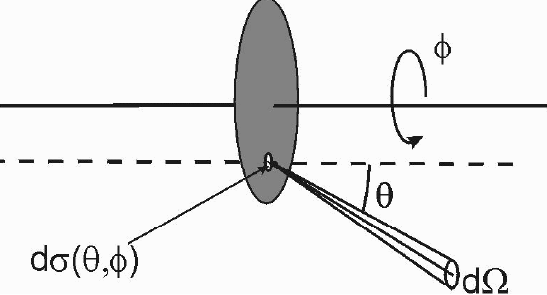
\includegraphics[width=0.8\linewidth]{introduction_and_review/dif_cross_sec.png}
    \caption{Differentiële cross sectie}%
    \label{fig:dif_cross_sec}
\end{figure}

De differentiële cross sectie is niets meer dan de cross sectie in functie van de ruimtehoek.
\begin{equation}
    \begin{aligned}
        \label{eq:dif_cross_sec}
        \sigma&=\int \left(\frac{d\sigma}{d\Omega}\right)d\Omega\\
        4\pi&=\int d\Omega\\
        d\Omega &= d\phi d\cos\theta = d\phi\sin\theta d\theta
    \end{aligned}
\end{equation}
Een botsing zal normaal de azimutale symmetrie behouden en krijgen we:
\begin{equation}
    \begin{aligned}
        \label{eq:dif_cross_sec_az_sym}
        \frac{d\sigma}{d\Omega}\rightarrow \frac{d\sigma}{d\cos\theta}
    \end{aligned}
\end{equation}
en is de $\phi$ afhankelijkheid irrelevant. Dit is niet het geval voor gepolariseerde bundels.\\

\subsection{Hoe meten we dit alles}%
\label{sub:hoe_meten_we_dit_alles}

Uit de experimenten hebben we het aantal deeltjes onder een bepaalde hoek $\theta$ gedetecteerd over de breedte van de hoek waaronder we waarnemen omdat deze eindig is. Deze willen we zo klein mogelijk. Uit al deze detecties moeten de deeltjes waarin we geïnteresseerd zijn, afgezonderd worden van de background deeltjes. Dit wordt weergegeven in de onderstaande vergelijkingen.
\begin{equation}
    \begin{aligned}
        \label{eq:measure_cros_sec}
        \frac{d\sigma}{d\cos\theta} &= \frac{\Delta N(\cos\theta)}{\Delta \cos\theta\cdot\mathcal{L}} \\
                                    &= \frac{\Delta N^{selected}(\cos\theta)-\Delta N_{background}^{expected}(\cos\theta)}{\mathcal{L}\cdot\Delta\cos\theta\cdot\epsilon(\cos\theta)} 
    \end{aligned}
\end{equation}
met $\epsilon$ de selectie efficiëntie. $\epsilon$ en $\Delta N_{background}^{expected}$ zullen bepaald worden in Monte Carlo berekeningen. Hierbij is het heel belangrijk om de trade-off tussen efficiëntie en background te optimaliseren.

\end{document}
